\subsubsection*{2.(1)}
ターンオフ動作
\subsubsection*{2.(2)}
図3に安全動作領域図を示す.
ここで線分PQは
\begin{align*}
  v=-\frac{3}{40}v+\frac{55}{2}
\end{align*}
であり$i=240$では$v=9.5$となる.したがってB点は安全動作領域外であり,デバイスは安全に動作しない.
\begin{figure}[htbp]
  \begin{center}
    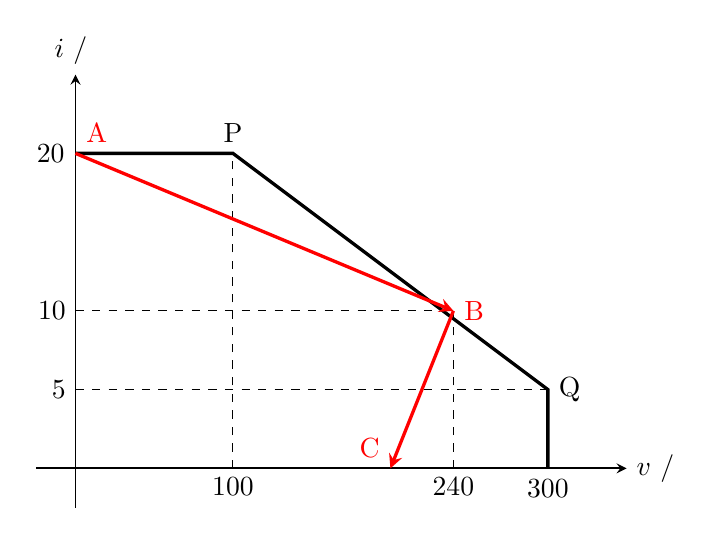
\begin{tikzpicture}
      \draw[->,>=stealth,semithick] (-0.5,0)--(7,0)node[right]{$v\ /\ \si{\volt}$}; %x軸
      \draw[->,>=stealth,semithick] (0,-0.5)--(0,5)node[above]{$i\ /\ \si{\ampere}$}; %y軸
      \draw[very thick] (0,4)node[left]{$20$}--(2,4)node[above]{P}--(6,1)node[right]{Q}--(6,0)node[below]{$300$};
      \draw[dashed, thin] (2,0)node[below]{$100$}--(2,4);
      \draw[dashed, thin] (0,1)node[left]{$5$}--(6,1);
      \draw[dashed, thin] (4.8,0)node[below]{$240$}--(4.8,2);
      \draw[dashed, thin] (0,2)node[left]{$10$}--(4.8,2);
      \draw[red, very thick,->,>=stealth] (0,4)node[above right]{A}--(4.8,2)node[right]{B};
      \draw[red, very thick,->,>=stealth] (4.8,2)--(4,0)node[above left]{C};
    \end{tikzpicture}
  \end{center}
  \caption{安全動作領域}
\end{figure}
\subsubsection*{2.(3)}
前問で得た式から線分PQの電流$10\ \si{\ampere}$における値は
\begin{align*}
  v=\frac{40}{3}\left(\frac{55}{2}-10\right)=\frac{700}{3}\ \si{\volt}\simeq233.3\ \si{\volt}
\end{align*}
である.したがって$v_{\rm ce}=233.3\ \si{\volt}$まで減少すれば安全に動作する.
そのときの安全動作領域図は図4である.
\begin{figure}[htbp]
  \begin{center}
    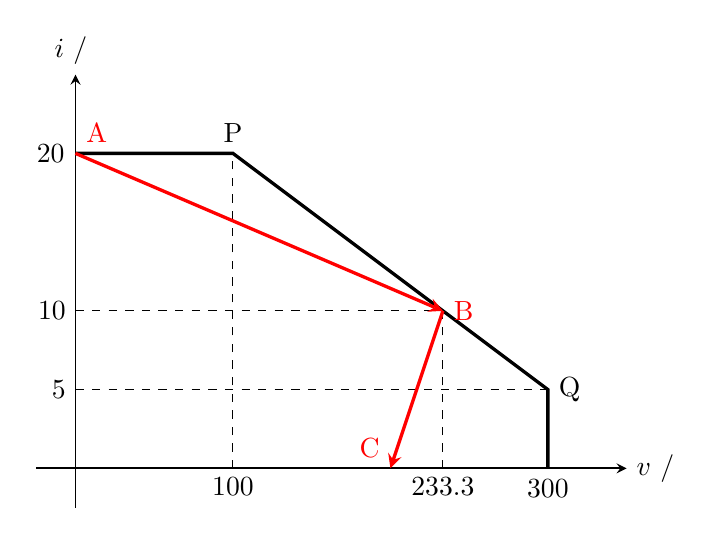
\begin{tikzpicture}
      \draw[->,>=stealth,semithick] (-0.5,0)--(7,0)node[right]{$v\ /\ \si{\volt}$}; %x軸
      \draw[->,>=stealth,semithick] (0,-0.5)--(0,5)node[above]{$i\ /\ \si{\ampere}$}; %y軸
      \draw[very thick] (0,4)node[left]{$20$}--(2,4)node[above]{P}--(6,1)node[right]{Q}--(6,0)node[below]{$300$};
      \draw[dashed, thin] (2,0)node[below]{$100$}--(2,4);
      \draw[dashed, thin] (0,1)node[left]{$5$}--(6,1);
      \draw[dashed, thin] ({14/3},0)node[below]{$233.3$}--({14/3},2);
      \draw[dashed, thin] (0,2)node[left]{$10$}--({14/3},2);
      \draw[red, very thick,->,>=stealth] (0,4)node[above right]{A}--({14/3},2)node[right]{B};
      \draw[red, very thick,->,>=stealth] ({14/3},2)--(4,0)node[above left]{C};
    \end{tikzpicture}
  \end{center}
  \caption{安全動作領域}
\end{figure}